\documentclass[12pt]{article}
\usepackage{stata}
\usepackage{graphicx}
\usepackage{geometry}
\usepackage{rotating}
\begin{document}



\author{Jesús Lara Jáuregui}
\title{Problem Set 1}
\maketitle



\section{Problem 1. OLS in MATA}
\subsection{Part 1}



\begin{stlog}. myreg1 lnwage hieduc exp exp2 
{\smallskip}
b[4,1]
            c1
r1   .08264541
r2   .02523881
r3  -.00037668
r4   1.3094414
{\smallskip}
symmetric V[4,4]
            c1          c2          c3          c4
r1   1.195e-06
r2   1.595e-07   .00001683
r3  -4.035e-09  -3.770e-07   8.579e-09
r4  -.00001749  -.00017676   3.899e-06   .00211062
{\smallskip}
\end{stlog}
/subsection{Part 2}
\begin{stlog}. quiet reg lnwage hieduc exp exp2
{\smallskip}
. matrix list e(b)
{\smallskip}
e(b)[1,4]
        hieduc         exp        exp2       _cons
y1   .08264541   .02523881  -.00037668   1.3094414
{\smallskip}
. matrix list e(V)
{\smallskip}
symmetric e(V)[4,4]
            hieduc         exp        exp2       _cons
hieduc   1.195e-06
   exp   1.595e-07   .00001683
  exp2  -4.035e-09  -3.770e-07   8.580e-09
 _cons   -.0000175  -.00017676   3.899e-06   .00211066
{\smallskip}
\end{stlog}

/section{Problem 2. Poisson using Maximum Likelihood}

If $y_i$ is distributed Poission with mean $exp(X^{'}_i /beta)$, hence the likelihood function for a sample of N observations is given by:

And taking logs we get:

\begin{stlog}. hist(num_awards), title("Number of Awards") color("orange")
(bin=14, start=0, width=.42857143)
{\smallskip}
\end{stlog}
\begin{center}
    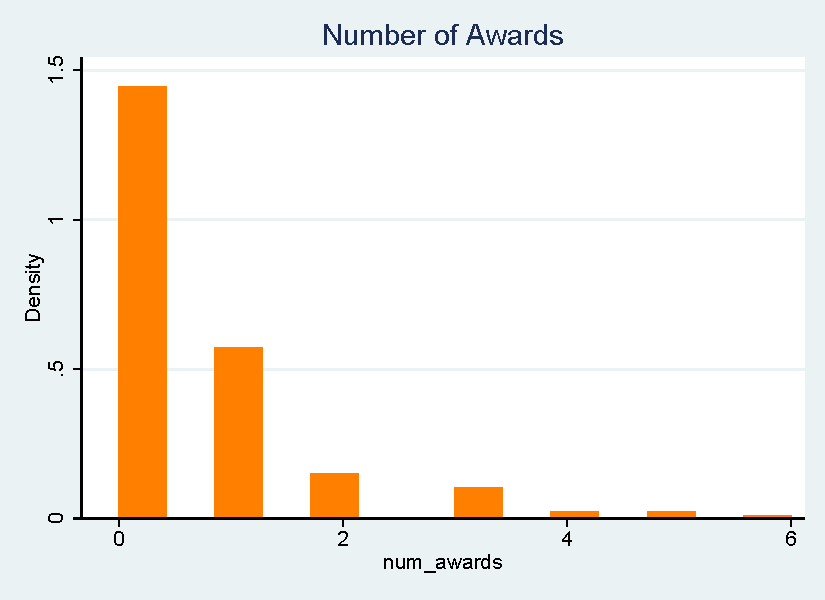
\includegraphics{797B_PS1_JL_3.pdf}
\end{center}

\end{document}

